% id: 0550
% book: 쎈 중3-2 수학 · 05 원주각의 활용
% section: 유형 08 접선과 현이 이루는 각
% figure: tikz:fig-0550
% answer: ③
% answer_source: 답지
% variant_level: 0 (원본 전사)
% 이 파일은 build.mjs 가 items.json 에서 만든다. 고칠 때는 items.json 을 고친다.
\smash{\raisebox{1.5mm}{\dmkichul{쎈 중3-2 수학 0550번 · 99쪽}}}
\noindent\begin{minipage}[t]{0.58\linewidth}\vspace{0pt}\raggedright 오른쪽 그림에서 $\triangle\pt{ABC}$는 원에 내접하고 직선~$\pt{CT}$는 원의 접선이다. $\arc{AB}:\arc{BC}:\arc{CA}=4:3:2$일 때, $\angle\pt{ACT}$의 크기는?\end{minipage}\hfill\begin{minipage}[t]{0.4\linewidth}\vspace{0pt}\centering \resizebox{\ifdim\width>\linewidth\linewidth\else\width\fi}{!}{% 0550(본책 99쪽) — 원에 내접하는 △ABC, 접선 CT(접점 C), 호 AB:BC:CA=4:3:2, ∠ACT 표시. 스캔 삽화를 TikZ 로 다시 그림.
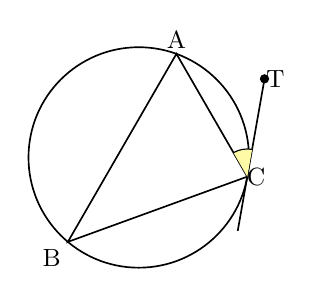
\begin{tikzpicture}[scale=1.4, line width=0.6pt]
  \draw (0.000,0.000) circle (1.000);
  \draw (0.342,0.940) -- (-0.643,-0.766) -- (0.985,-0.174) -- cycle;
  \draw (0.898,-0.666) -- (1.141,0.713);
  \fill[yellow!35] (0.985,-0.174) -- ++(80.000:0.250) arc[start angle=80.000, end angle=120.000, radius=0.250] -- cycle;
  \draw[line width=0.4pt] (1.028,0.073) arc[start angle=80.000, end angle=120.000, radius=0.250];
  \fill (1.141,0.713) circle (1.2pt);
  \node[font=\small, anchor=west, inner sep=1.5pt] at (1.111,0.713) {T};
  \node[font=\small, anchor=south, inner sep=1.5pt] at (0.342,0.940) {A};
  \node[font=\small, anchor=north east, inner sep=1.5pt] at (-0.663,-0.786) {B};
  \node[font=\small, anchor=west, inner sep=1.5pt] at (0.935,-0.174) {C};
\end{tikzpicture}
}\end{minipage}\par
\begin{choicesii}{$35^\circ$}{$38^\circ$}{$40^\circ$}{$42^\circ$}{$45^\circ$}\end{choicesii}
